\boxde
\BTTN
\Opensolutionfile{ans}[ans/2D1-2-DEON-5]
\begin{ex}
    \immini{Cho hàm số $y=f\left(x\right)$ có bảng biến thiên như sau. Hàm số đã cho nghịch biến trên khoảng nào dưới đây?
        \choice
        {$\left(1;+\infty\right)$}
        {\True $\left(0;1\right)$}
        {$\left(-\infty;0\right)$}
        {$\left(-1;0\right)$}}{
        
\begin{tikzpicture}
            \tkzTabInit[nocadre=false,lgt=1.1,espcl=1.5,deltacl=0.6]
            {$x$ /0.6,$y'$ /0.6,$y$ /2.2}
            {$-\infty$,$-1$,$0$,$1$,$+\infty$}
            \tkzTabLine{,-,$0$,+,$0$,-,$0$,+,}
            \tkzTabVar{+/$+\infty$, -/$-2$,+/$3$,-/$-2$,+/$+\infty$}
    \end{tikzpicture}}
    \loigiai{
        Dựa vào bảng biến thiên ta suy ra hàm số đã cho nghịch biến trên khoảng $\left(0;1\right)$.
    }
\end{ex}

\begin{ex}%[2D1H1-3]
    \immini{Cho hàm số $y=f(x)$ xác định liên tục và liên tục trên $\mathbb{R}$ và có bảng biến thiên như sau. Khẳng định nào sau đây đúng?
        \choice
        {Hàm số có $2$ cực trị}
        {Hàm số có giá trị cực đại bằng $2$}
        {\True Hàm số có giá trị cực tiểu bằng $0$}
        {Hàm số có giá trị cực đại tại $x=0$}}{
        
\begin{tikzpicture}
            \tkzTabInit[nocadre = false,lgt = 1,espcl =3]
            {$x$  /0.7,  $y'$  /0.7,  $y$  /2.2}{  $-\infty$  ,  $2$  ,  $+\infty$}
            \tkzTabLine{,-,  $0$  ,+,}
            \tkzTabVar{+/  $+\infty$, -/$0$, +/  $+\infty$  }
    \end{tikzpicture}}
    \loigiai{Dựa vào bảng biến thiên, ta thấy hàm số đạt cực tiểu tại $x=2$ và $y=0$. Do đó, giá trị cực tiểu của hàm số bằng $0$.}
\end{ex}

\begin{ex}%[2D1H1-3]
    \immini{Cho hàm số $y=f(x)$ có bảng biến thiên như sau. Tìm giá trị cực đại $y_{\text{CĐ}}$ và giá trị cực tiểu $y_{\text{CT}}$ của hàm số đã cho.
        \choice
        {$y_{\text{CĐ}}=3$ và $y_{\text{CT}}=2$}
        {$y_{\text{CĐ}}=2$ và $y_{\text{CT}}=0$}
        {$y_{\text{CĐ}}=3$ và $y_{\text{CT}}=3$}
        {\True $y_{\text{CĐ}}=3$ và $y_{\text{CT}}=0$}}{
        
\begin{tikzpicture}
            \tkzTabInit[nocadre = false,lgt = 1,espcl = 2]
            {  $x$  /0.7,  $y'$  /0.7,  $y$  /2}{  $-\infty$  , $0$,  $2$  ,  $+\infty$  }
            \tkzTabLine{ ,+, $0$, -,  $0$  ,+,}
            \tkzTabVar{-/  $-\infty$ ,+/  $3$  ,-/  $0$  , +/  $+\infty$  }
    \end{tikzpicture}}
    \loigiai{
        Dựa vào bảng biến thiên ta có $y_{\text{CĐ}}=3$ và $y_{\text{CT}}=0$.
    }
\end{ex}

\begin{ex}
    \immini{Cho hàm số $y=f(x)$ xác định trên $\mathbb{R} \setminus \{0\}$, liên tục trên mỗi khoảng xác định và có bảng biến thiên như hình bên. Hàm số đã cho có bao nhiêu điểm cực trị?
        \choice
        {\True $ 1 $}
        {$ 0 $}
        {$ 3 $}
        {$ 2 $}}{
        
\begin{tikzpicture}
            \tikzset{double style/.append style = {draw=\tkzTabDefaultWritingColor,double=\tkzTabDefaultBackgroundColor,double distance=2pt}}
            \tkzTabInit[nocadre=false,lgt=1.2,espcl=1.9,deltacl=0.6]
            {$x$/0.6,$y'$/0.6,$y$/2}
            {$-\infty$,$0$,$1$,$+\infty$}
            \tkzTabLine{ ,-,d,+,0,-, }
            \tkzTabVar{+/$+\infty$,-D-/ $-1$ / $-\infty$ ,+/$2$,-/$-\infty$}
    \end{tikzpicture}}
    \loigiai{
        Dựa vào bảng biến thiên ta thấy hàm số chỉ đạt cực trị tại $x=1$.\\
        Vậy hàm số có một cực trị.
    }
\end{ex}

\begin{ex}
    \immini{Cho hàm số bậc ba $y=f(x)$ có đồ thị như hình vẽ bên. Mệnh đề nào sau đây đúng?
        \choice
        {Hàm số nghịch biến trên $(-\infty; +\infty)$}
        {Hàm số đồng biến trên $(-\infty; 2)$}
        {\True Hàm số đồng biến trên $(-\infty; -1)$}
        {Hàm số nghịch biến trên $(1; +\infty)$}
    }
    {

        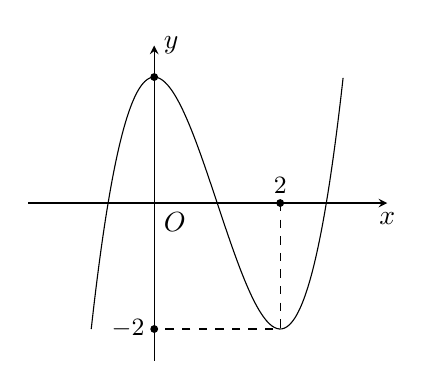
\begin{tikzpicture}[smooth,samples=300,scale=0.8,>=stealth]
            \draw[->] (-2,0)--(3.7,0) node[below]{$x$};
            \draw[->] (0,-2.5)--(0,2.5) node[right]{$y$};
            \draw (0,0) node[below right]{$O$};
            \draw[smooth,samples=100,domain=-1:3]
            plot(\x,{(\x)^3-3*(\x)^2+2});
            \draw[fill=black] (2,0) circle(1.5pt) (0,2) circle(1.5pt) (0,-2) circle(1.5pt);
            \draw[dashed] (2,0)node[above]{\small$2$}--(2,-2)--(0,-2)node[left]{\small$-2$};
        \end{tikzpicture}
    }

    \loigiai{Dựa vào đồ thị ta thấy: Trên khoảng $(-\infty; -1)$, đồ thị là đường liền đi lên kể từ trái qua phải, nên hàm số đồng biến trên $(-\infty; -1)$.
    }

\end{ex}

\begin{ex}%[2D1N1-1]
    Cho hàm số $y=\dfrac{x+1}{x-3}$. Trong các mệnh đề sau, mệnh đề nào \textbf{sai}?
    \choice
    {Hàm số nghịch biến trên từng khoảng xác định của nó}
    {\True Hàm số nghịch biến trên tập xác định của nó}
    {Hàm số nghịch biến trên khoảng $(3;+\infty)$}
    {Hàm số nghịch biến trên khoảng $(-\infty; 3)$}
    \loigiai{Hàm số đã cho có tập xác định gồm hai khoảng $(-\infty; 3)$ và $(3;+\infty)$ rời nhau nên khẳng định hàm số nghịch biến trên tập xác định là sai.}
\end{ex}

\begin{ex}%[2D1H1-1]
    Hàm số nào sau đây \textbf{không} đồng biến trên $(-\infty;+\infty)$
    \choice
    {$y=x^5+x^3-1$}
    {$y=x^3+2$}
    {\True $y=\dfrac{x-1}{x+2}$}
    {$y=x+1$}
    \loigiai{
        Ta có $y=\dfrac{x-1}{x+2}\Rightarrow y'=\dfrac{3}{{(x+2)}^2} > 0,\forall x\ne-2$. \\
        Do đó hàm số đồng biến trên các khoảng $(-\infty;2)$ và $(2;+\infty)$.}
\end{ex}

\begin{ex}
    Tìm khoảng đồng biến của hàm số $y=-x^3+3x^2-1$.
    \choice
    {$(-2;0)$}
    {\True $(0;2)$}
    {$(-1;3)$}
    {$(0;3)$}
    \loigiai{
        Ta có $y'=-3x^2+6x$. Do đó $y'>0\Leftrightarrow -3x^2+6x>0\Leftrightarrow 0<x<2$.\\
        Vậy hàm số đồng biến trên khoảng $(0;2)$.
    }
\end{ex}


\begin{ex}%[2D1N1-1]
    Các khoảng đồng biến của hàm số $y=x^4-8x^2-4$ là
    \choice
    {$(-\infty;-2)$ và $(2;+\infty)$}
    {$(-2;0)$ và $(0;+\infty)$}
    {$(-\infty;-2)$ và $(0;2)$}
    {\True $(-2;0)$ và $(2;+\infty)$}
    \loigiai{Ta có tập xác định của hàm số là $\mathscr{D}=\mathbb{R}$ và $y'=4x^3-16x$ nên $y'=0\Leftrightarrow
        \hoac{&x=0\\
            &x=-2\\
            &x=2.}$ \\
        Khi đó $y'\ge 0\Leftrightarrow 4x^3-16x\ge 0\Leftrightarrow \hoac{&x\ge 0\\
            &-2\le x\le 0.}$ \\
        Vậy hàm số đồng biến trên các khoảng $(-2;0)$ và $(2;+\infty)$.
    }
\end{ex}

\begin{ex}%[TT Lần 1, SGD Ninh Bình, 2018-2019]%[Vũ Nguyễn Hoàng Anh, 12EX6]%[2D2B4-3]%
    Cho hàm số $f(x)=\ln x-x$. Khẳng định nào dưới đây đúng?
    \choice
    {Hàm số đồng biến trên khoảng  $(0;+\infty)$}
    {Hàm số đồng biến trên các khoảng  $(-\infty;0)$ và $(1;+\infty)$}
    {\True Hàm số đồng biến trên khoảng  $(0;1)$}
    {Hàm số đồng biến trên khoảng $(1;+\infty)$}
    \loigiai{
        Tập xác định của hàm số là $\mathscr{D}=(0;+\infty)$. Ta có
        $$f'(x)=\dfrac{1}{x}-1=\dfrac{1-x}{x}\quad \text{và}\quad  f'(x)=0 \Leftrightarrow x=1.$$
        Bảng xét dấu đạo hàm của hàm $y=f(x)$
        \begin{center}
            \begin{tikzpicture}
                \tkzTabInit[nocadre=false, lgt=1.5, espcl=2]{$x$ /0.7,$f'(x)$ /0.7}
                {$0$,$1$,$+\infty$}
                \tkzTabLine{,+,$0$,-,}
            \end{tikzpicture}
        \end{center}
        Hàm số đồng biến trên khoảng $(0;1)$.
    }
\end{ex}

\begin{ex}%[KSCL tháng 3, Trần Phú-Yên Lạc, Vĩnh Phúc, 2018]%[2D2B4-3]%[Đức Nguyễn, dự án 12EX-8]%
    Điểm cực đại của hàm số $y=(2x+1)\mathrm{e}^{1-x}$ là
    \choice
    {$x=\dfrac{3}{2}$}
    {$x=1$}
    {$x=-1$}
    {\True $x=\dfrac{1}{2}$}
    \loigiai{
        Ta có $y'=(2x+1)'\mathrm{e}^{1-x}+\left(2x+1\right)\left(\mathrm{e}^{1-x}\right)'=(-2x+1)\mathrm{e}^{1-x}$.\\
        $y'=0\Leftrightarrow x=\dfrac{1}{2}$.\\
        Bảng biến thiên của hàm số
        \begin{center}
            \begin{tikzpicture}
                \tkzTabInit[lgt=1.2,espcl=3]
                {$x$  /1.2, $y'$ /1.2,$y$  /2.0}
                {$-\infty$ , $\dfrac{1}{2}$, $+\infty$}
                \tkzTabLine{,+,z,-,}
                \tkzTabVar{-/$-\infty$ ,+/$y_\text{CĐ}$,-/$-\infty$}
            \end{tikzpicture}
        \end{center}
        Vậy hàm số đạt cực đại tại $x=\dfrac{1}{2}$.
    }
\end{ex}

\begin{ex}%2D1B5-5]
    \immini{Cho hàm số bậc bốn $y=f(x)$ có đồ thị hàm số $y=f'(x)$ như hình vẽ dưới. Hàm số $y=f(x)$ đồng biến trên khoảng nào?
        \haicot
        {$(-\infty;0)$}
        {\True $(-3;+\infty)$}
        {$(-\infty;4)$}
        {$(-4;0)$}
    }{	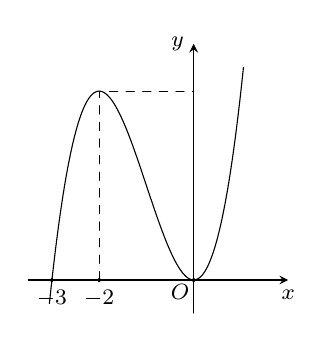
\begin{tikzpicture}[scale=0.6, font=\footnotesize, line join=round, line cap=round, >=stealth]
            \draw[->] (-3.5,0)--(2,0) node[below] {$x$};
            \draw[->] (0,-0.7)--(0,5) node[left] {$y$};
            \draw[fill=black] (0,0) circle (1pt) node[below left=-2pt] {$O$};
            \draw[fill=black] (-2,0) circle (1pt) node[below] {$-2$};
            \draw[fill=black] (-3,0) circle (1pt) node[below] {$-3$};
            \draw[dashed] (-2,0)--(-2,4)--(0,4);
            \clip (-3.5,-0.5) rectangle (2,4.5);
            \draw[smooth,samples=100,domain=-3.5:2] plot(\x,{(\x)^3+3*(\x)^2});
    \end{tikzpicture}}
    \loigiai{
        Dựa vào đồ thị hàm số $y=f'(x)$ ta thấy $f'(x) \geqslant 0, \forall x \in (-3;+\infty)$, suy ra hàm số $y=f(x)$ đồng biến trên khoảng $(-3;+\infty)$.
    }

\end{ex}

\begin{ex}
    Cho hàm số $y=f(x)$ có $ f'(x)=x^2(x-1)^3(3-x)(x-5)$. Số điểm cực tiểu của đồ thị hàm số là
    \choice
    {$4$}
    {$2$}
    {$3$}
    {\True $1$}
    \loigiai{
        Ta có
        $f'(x)=0\Leftrightarrow x^2(x-1)^3(3-x)(x-5)=0\Leftrightarrow\hoac{&x=0 \text{ (bội 2)}\\&x=1 \text{ (bội 3)}\\&x=3\\&x=5.}$\\
        Ta có bảng xét dấu của $f'(x)$
        \begin{center}
            \begin{tikzpicture}
                \tkzTabInit[nocadre=false,lgt=1.2,espcl=2.5,deltacl=0.6]
                {$x$ /0.6,$f'(x)$ /0.6}
                {$-\infty$ , $0$, $1$, $3$, $5$, $+\infty$}
                \tkzTabLine{,+,0,+,0,-,0,+,0,-,}
            \end{tikzpicture}
        \end{center}
        Dựa vào bảng xét dấu ta thấy đồ thị hàm số $y=f(x)$ có $1$ điểm cực tiểu.}
\end{ex}

\begin{ex}%[Đề thi thử THPTQG lần 1, Quỳnh Lưu 1, Nghệ An 2018]%[Lê Đình Mẫn, Dự án EX6]%[2D1B2-1]%
    Đồ thị hàm số $y=2x^3-6x^2-18x$ có hai điểm cực trị $A$ và $B$. Điểm nào dưới đây thuộc đường thẳng $AB$?
    \choice
    {\True $E(1;-22)$}
    {$H(1;-10)$}
    {$K(0;6)$}
    {$G(3;54)$}
    \loigiai{
        Ta có $y'=6x^2-12x-18$; $y'=0 \Leftrightarrow x=-1$ hoặc $x=3$.\\
        Tọa độ hai điểm cực trị là $A(-1;10)$ và $B(3;-54)$. Đường thẳng $AB$ có dạng
        $$\dfrac{x-x_A}{x_B-x_A}=\dfrac{y-y_A}{y_B-y_A} \Leftrightarrow \dfrac{x+1}{4}=\dfrac{y-10}{-64} \Leftrightarrow y=-16x-6.$$
        Trong $4$ điểm thì chỉ có điểm $E(1;-22)$ thuộc đường thẳng đó.
    }
\end{ex}

\begin{ex}%[2D1V1-1]
    Tất cả các giá trị của tham số $m$ sao cho hàm số $y=-x^3-3mx^2+4m-1$ đồng biến trên khoảng $(0;4)$ là
    \choice
    {$-2\leqslant m < 0$}
    {$m\leqslant-4$}
    {\True $m\leqslant-2$}
    {$m > 0$}
    \loigiai{
        Ta có $y'=-3x^2-6mx$. Cho $y'=0\Leftrightarrow
        \left[\begin{aligned}
            &x=0\\
            &x=-2m.
        \end{aligned}\right.$\\
        Nếu $m=0$ thì hàm số nghịch biến trên $\mathbb{R}$ (không thỏa mãn yêu cầu bài toán). \\
        Với $m\neq 0$: Giả sử $\{x_1;x_2\}=\{0;-2m\}$. Yêu cầu bài toán thỏa mãn khi bảng biến thiên của hàm số như sau
        \begin{center}
            
\begin{tikzpicture}
                \tkzTabInit[nocadre = false,lgt = 1,espcl =2.3]
                {  $x$  /0.7,  $y'$  /0.7,  $y$  /2}{  $-\infty$  ,  $0$, $-2m$ ,  $+\infty$  }
                \tkzTabLine{,+,$0$,-,  $0$  ,+,}
                \tkzTabVar{-/  $-\infty$  ,+/  $-1$ , -/$y(-2m)$  , +/  $+\infty$  }
            \end{tikzpicture}
        \end{center}
        và
        $$ \left\{\begin{aligned}	& x_1=0\\
            &x_2=-2m \geqslant 4\end{aligned}\right. \Leftrightarrow m \leqslant-2. $$
    }
\end{ex}
\Closesolutionfile{ans}

\BTTF
\Opensolutionfile{ans}[ans/B1-De2-2]

\begin{ex}%[2D1H1-1]
    Cho hàm số $y=f(x)$ liên tục trên $\mathbb{R}$ và có bảng biến thiên như hình vẽ.
    \begin{center}
        \begin{tikzpicture}
            \tkzTabInit[lgt = 1.5,espcl = 3]%
            {$x$ /0.7, $f'(x)$/0.8}
            {$-\infty$ ,  $-1$,  $1$,  $+\infty$  }
            \tkzTabLine{ ,+,0,-,0,+,}
        \end{tikzpicture}
    \end{center}
    Xét tính đúng, sai của các mệnh đề sau:
    \choiceTF
    {\True Hàm số có $2$ điểm cực trị}
    {\True Hàm số nghịch biến trên khoảng $(-1;1)$}
    {\True Hàm số đồng biến trên khoảng $(1;+\infty)$}
    {Hàm số $f(1-x)$ nghịch biến trên khoảng $(-1;1)$}
    \loigiai
    {Dựa vào bảng biến của hàm số $y=f(x)$ ta có
        \begin{itemchoice}
            \itemch Hàm số đạt cực đại tại $x=-1$ và đạt cực tiểu tại $x=1$.
            \itemch Hàm số nghịch biến trên khoảng $(-1;1)$.
            \itemch Hàm số đồng biến trên khoảng $(1;+\infty)$.
            \itemch Đặt $g(x)=f(1-x)$. Ta có
            \begin{itemize}
                \item [$\bullet$] $g'(x)=-f'(1-x)$; \\
                $g'(x)=0 \Leftrightarrow f'(1-x)=0 \Leftrightarrow \hoac{&1-x=-1\\&1-x=1}\Leftrightarrow \hoac{&x=2\\&x=0.}$
                \item [$\bullet$] Bảng biến thiên hàm $g(x)=f(1-x)$:
                \begin{center}
                    \begin{tikzpicture}
                        \tkzTabInit[lgt=1.2,espcl=2]
                        {$x$ /0.7, $g'(x)$ /0.7, $g(x)$ /2}
                        {$-\infty$,$0$,$2$,$+\infty$}
                        \tkzTabLine{,-,$0$,+,$0$,-,}
                        \tkzTabVar{+/,-/,+/,-/}
                    \end{tikzpicture}
                \end{center}
                Hàm số $g(x)$ nghịch biến trên các khoảng $(-\infty;0)$ và $(2;+\infty)$.
            \end{itemize}
        \end{itemchoice}
    }
\end{ex}

\begin{ex}%[2D1H1-4]
    \immini{Cho hàm số $y=f(x)$ xác định và liên tục trên đoạn $\left[0 ; \dfrac{16}{5}\right]$ thoả mãn\\
        $f'\left(\dfrac{1}{3}\right)=f'(1)=f'\left(\dfrac{5}{2}\right)=0$ và có đồ thị là đường cong như hình bên. Xét tính đúng sai của các mệnh đề sau:
        \choiceTF
        {\True $x=1$ là điểm cực đại của hàm số}
        {\True $x=\dfrac{1}{3}$, $x=\dfrac{5}{2}$ là điểm cực tiểu của hàm số}
        {Hàm số đã cho nghịch biến trên $\left(\dfrac{1}{3};1\right)$ và $\left(\dfrac{5}{2};+\infty\right)$}
        {Đồ thị có điểm cực đại là $\left(\dfrac{16}{5};3 \right)$ }}{
        \begin{tikzpicture}[y=1.2cm,line cap=butt,line join=miter,>=stealth,font=\footnotesize,scale=.7]
            \tikzset{declare function={xmin=-1.5;xmax=4.5;ymin=-2.3;ymax=3;
                    f(\x)=32/45*(\x)^4-32/9*(\x)^3+224/45*(\x)^2-32/15*(\x);
                },
                smooth,samples=250
            }
            \draw[->] (xmin,0)--(xmax,0) node[shift={(-100:7pt)}]{$ x $};
            \draw[->] (0,ymin)--(0,ymax) node[shift={(10:7pt)}]{$ y $};
            \fill (0,0) node[shift={(135:10pt)}]{$ O $};
            \draw[dashed](1/3,0)node[shift={(90:8pt)}]{$\tfrac{1}{3}$}|-(0,-1/3.5)node[shift={(-150:9pt)}]{$-\tfrac{1}{3}$}
            (2.5,0)node[shift={(90:7pt)}]{$\tfrac{5}{2}$}|-(0,-2)node[shift={(180:9pt)}]{$-2$}	(1,0)node[shift={(90:7pt)}]{$1$}
            (3.2,0) node[shift={(-90:7pt)},font=\scriptsize]{$\tfrac{16}{5}$} |-(0,{f(3.2)}) node[shift={(180:7pt)}]{$3$};
            \clip (xmin,ymin) rectangle (xmax,ymax);
            \draw  plot[domain=0:3.2] (\x, {f(\x)});
    \end{tikzpicture}}
    \loigiai{
        Theo hình vẽ đồ thị thì
        \begin{itemchoice}
            \itemch $x=1$ là điểm cực đại của hàm số.
            \itemch $x=\dfrac{1}{3}$, $x=\dfrac{5}{2}$ là điểm cực tiểu của hàm số.
            \itemch Hàm số đã cho nghịch biến trên $\left(-\infty;\dfrac{1}{3}\right)$ và $\left(1;\dfrac{5}{2}\right)$.
            \itemch Không thể khẳng định đồ thị có điểm cực đại là $\left(\dfrac{16}{5};3 \right)$.
    \end{itemchoice}}
\end{ex}

\begin{ex}%[2D1H2-2]
    \immini{Cho hàm số $y=f(x)$ có đồ thị $f'(x)$ trên $[2;5]$ như hình bên. Xét tính đúng sai của các mệnh đề sau:
        \choiceTF
        {Hàm số đạt cực tiểu tại $x=-1$}
        {\True Hàm số đồng biến trên $(-1;2)$ và $(4;5)$}
        {Hàm số nghịch biến trên $(2;4)$}
        {\True Hàm số $f(x+2)$ đạt cực đại tại $x=0$}}{
        \begin{tikzpicture}[scale=0.7, font=\footnotesize, line join=round, line cap=round, >=stealth]
            \def\a{0.125} \def\b{-0.625} \def\c{0.25} \def\d{1} % Hệ số
            \def\xt{-3} \def\xp{6} \def\yt{3} \def\yd{-3} % x_trái, x_phải, y_trên, y_dưới (giới hạn)
            \draw[->] (\xt,0)--(\xp,0) node [below]{$x$};
            \draw[->] (0,\yd)--(0,\yt) node [left]{$y$};
            \node at (0,0) [below right]{$O$};
            \draw[smooth,samples=200,domain=-2:5] plot(\x,{\a*(\x)^3+\b*(\x)^2+\c*(\x)+\d}) node [above right]{$y=f'(x)$};
            \draw[dashed] (-2,0) node [below left]{$-2$} -- (-2,-3)
            (5,0) node [below]{$5$} -- (5,2.25);
            \fill (-1,0) circle (1.5pt) node[above]{$-1$}
            (2,0) circle (1.5pt) node[above]{$2$}
            (4,0) circle (1.5pt) node[above]{$4$};
    \end{tikzpicture}}
    \loigiai{
        Từ đồ thị ta thấy $f'(x)=0 \Leftrightarrow \hoac{& x=-1\\ & x=2\\ & x=4.}$\\
        Ta có bảng biến thiên như sau
        \begin{center}
            \begin{tikzpicture}
                \tkzTabInit[nocadre=true,lgt=1.2,espcl=2.5,deltacl=0.6]
                {$x$ /0.6,$f'(x)$ /0.6,$f(x)$ /2}
                {$-2$,$-1$,$2$,$4$,$5$}
                \tkzTabLine{,-,$0$,+,$0$,-,$0$,+,}
                \tkzTabVar{+/,-/,+/,-/,+/}
            \end{tikzpicture}
        \end{center}
        \begin{itemchoice}
            \itemch Hàm số đạt cực tiểu tại $x=-1$, $x=4$.
            \itemch Hàm số đồng biến trên $(-1;2)$ và $(4;5)$.
            \itemch Hàm số nghịch biến trên $(-2;-1)$ và $(2;4)$.
            \itemch Hàm số $f(x)$ đạt cực đại tại $x=2$. Suy ra hàm số $f(x+2)$ đạt cực đại tại $x=0$.
        \end{itemchoice}
    }
\end{ex}

\begin{ex}
    Cho hàm số $y=x-\ln(1+x)$. Xét tính đúng sai của các mệnh đề sau:
    \choiceTF
    {\True Hàm số có tập xác định là $(-1;+\infty)$}
    {Hàm số đồng biến trên $(-1;+\infty)$}
    {\True Hàm số đạt cực tiểu tại điểm $x=0$}
    {Hàm số đồng biến trên $(-1;0)$}
    \loigiai{
        \begin{itemchoice}
            \itemch Điều kiện $1+x>0 \Leftrightarrow x>-1$. Suy ra tập xác định $\mathscr{D}=(-1;+\infty)$.
            \itemch Ta có $y'=1-\dfrac{1}{1+x}=\dfrac{x}{1+x}$;\quad $y'=0\Leftrightarrow x=0$.\\
            Bảng biến thiên trên miền $(-1;+\infty)$:
            \begin{center}
                
\begin{tikzpicture}
                    \tkzTabInit[nocadre=false,lgt=1,espcl=2.5]
                    {$x$ /0.6,$y'$ /0.6,$y$ /2}
                    {$-1$,$0$,$+\infty$}
                    \tkzTabLine{,-,$0$,+,}
                    \tkzTabVar{+/, -/$0$,+/}
                \end{tikzpicture}
            \end{center}
            Suy ra hàm số đồng biến trên $(0;+\infty)$.
            \itemch  Dựa vào bảng xét dấu suy ra hàm số đạt cực tiểu tại $x=0$.
            \itemch  Trên khoảng $(-1;0)$ thì hàm số nghịch biến.
        \end{itemchoice}
    }
\end{ex}
\Closesolutionfile{ans}

\BTTL
\Opensolutionfile{ans}[ans/B1-De2-3]
\begin{ex}%[2D1H1-1]
    Hàm số $y=\dfrac{1}{4}x^4-\dfrac{1}{2}x^3$ có bao nhiêu điểm cực trị?
    \shortans{$1$}
    \loigiai{Ta có $y'=x^3-\dfrac{3}{2}x^2=x^2\left(x-\dfrac{3}{2}\right)$ chỉ đổi dấu khi qua điểm $x=\dfrac{3}{2}$ nên hàm số có 1 điểm cực trị.}
\end{ex}

\begin{ex}
    Cho hàm số $y=f(x)=\dfrac{-3 x^2-5 x-5}{x-2}$. Gọi $x_1$, $x_2$ là hai điểm cực trị của hàm số đã cho. Tính $x_1+x_2$.
    \shortans{$4$}
    \loigiai{
        Tập xác định $D=\mathbb{R} \backslash\{2\}$.\\
        Đạo hàm $y'=\dfrac{-3x^2+12x+15}{(x-2)^2}$.\\
        $y'=0 \Leftrightarrow -3x^2+12x+15 =0$. Phương trình này luôn có hai nghiệm phân biệt $x_1$, $x_2$.\\
        Áp dụng định lý Viet, ta được $x_1+x_2=-\dfrac{b}{a}=\dfrac{-12}{-3}=4$.
    }
\end{ex}

\begin{ex}%[2D1V1-1]
    Gọi $A$, $B$ là hai điểm cực trị của đồ thị hàm số $y=x^3-3x^2+4$. Tính diện tích $S$ của tam giác $OAB$ với $O$ là gốc tọa độ.
    \shortans{$4$}
    \loigiai{
        Ta có $y'=3x^2-6x$ và $y'=0\Leftrightarrow x=0$ hoặc $x=2$.\\
        Do đó hai điểm cực trị của đồ thị hàm số là $A(0;4), B(2;0)$.\\
        Diện tích tam giác vuông $OAB$ là $S_{\triangle OAB}=\dfrac{1}{2}OA\cdot OB=4$.
    }
\end{ex}


\begin{ex}%[2D1H1-3]
    Cho hàm số $y=\dfrac{mx+2}{2x+m}$, $m$ là tham số thực. Gọi $S$ là tập hợp tất cả các giá trị nguyên của $m$ để hàm số nghịch biến trên khoảng $(0;1)$. Tìm số phần tử của $S$.
    \shortans{$2$}
    \loigiai{$y'=\dfrac{m^2-4}{(2x+m)^2}$.\\
        Hàm số nghịch biến trên khoảng $(0;1)$ khi và chỉ khi
        \[\heva{&m^2-4< 0\\
            &-\dfrac{m}{2}\notin (0;1)}\Leftrightarrow \heva{&-2< m < 2\\
            &\hoac{&m\ge 0\\
                &m\le-2}}\Leftrightarrow 0\le m < 2.\]
        Vậy số phần tử của tập $S$ là $2$.
    }
\end{ex}


\begin{ex}%[2D1V1-1]
    Tìm giá trị của tham số $m$ để hàm số $f(x)=(m^2-3)x-2m\ln{x}$ đạt cực tiểu tại điểm $x_0=1$.
    \shortans{$3$}
    \loigiai{
        Ta có $f'(x)=m^2-3-2m \cdot \dfrac{1}{x}$. \\
        Nhận thấy hàm số có đạo hàm tại $x_0=1$. Do đó, hàm số đạt cực trị tại $x_0=1$ khi
        \[ f'(1)=0\Leftrightarrow m^2-3-2m=0\Leftrightarrow \hoac{	&m=-1\\
            &m=3.}\]
        Khi $m=-1$ thì $f'(x)=-2+\dfrac{2}{x}$. Kiểm tra được $\heva{&f'(0.98)>0\\&f'(1,02)<0}$ nên lúc này $x=1$ là điểm cực đại.\\
        Khi $m=3$ thì $f'(x)=6-\dfrac{6}{x}$. Kiểm tra được $\heva{&f'(0.98)<0\\&f'(1,02)>0}$ nên lúc này $x=1$ là điểm cực tiểu.\\
        Vậy $m=3$.
    }
\end{ex}


\begin{ex}%[2D1C1-1]
    Gọi $(P)$ là parabol qua 3 điểm cực trị của đồ thị hàm số $y=\dfrac{1}{4}x^4-mx^2+m^2$. Tìm tất cả các giá trị thực của tham số $m$ để $(P)$ qua $A(2;24)$.
    \shortans{$6$}
    \loigiai{$y'=x^3-2mx$, $y'=0\Leftrightarrow\hoac{&x=0\\
            &x^2=2m.}$\\
        Để đồ thị hàm số có ba cực trị thì $m > 0$.\\
        $y'=0\Leftrightarrow\hoac{	&x=0\Rightarrow y=m^2\\
            &x=\pm\sqrt{2m}\Rightarrow y=0.}$\\
        Vậy ba điểm cực trị của đồ thị hàm số là $A(0;m^2)$, $B(\sqrt{2m};0)$, $C(-\sqrt{2m};0)$.\\
        Gọi $(P)\colon y=ax^2+bx+c$ là parabol qua ba cực trị của đồ thị hàm số.\\
        $\Rightarrow\heva{&c=m^2\\
            &2ma+b\sqrt{2m}+c=0\\
            &2ma-b\sqrt{2m}+c=0}\Leftrightarrow\heva{&c=m^2\\
            &a=-\dfrac{m}{2}\\
            &b=0}\Rightarrow y=-\dfrac{m}{2}x^2+m^2$.\\
        Để $(P)$ đi qua $A(2;24)$ thì $24=-\dfrac{m}{2}\cdot4+m^2\Leftrightarrow m^2-2m-24=0\Leftrightarrow\hoac{&m=6\\
            &m=-4.}$ \\
        Do $m > 0$ nên nhận $m=6$.
    }
\end{ex}
\Closesolutionfile{ans}
%\indapan{10}{ans/2D1-2-DEON-5}